% Figure 0 - Mechanism schematic (paper visual anchor).
% Na_xCoO2.yH2O: how CoO2-CoO2 spacing (hydration) drives the alkali gallery
% mode from a stiff single well (no 2DEG) through a soft double well (2DEG on,
% SC window) to a deep polaronic double well at the bilayer spacing.
% Build:  pdflatex fig0_schematic.tex
\documentclass[border=4pt]{standalone}
\usepackage{tikz}
\usepackage{amsmath}
\usetikzlibrary{arrows.meta,positioning,decorations.pathreplacing,
                decorations.pathmorphing,patterns,backgrounds,fit,calc}

% ---- palette (didactic; distinct from the data-plot series colours) ----
\definecolor{slab}{HTML}{3C6E82}   % CoO2 slab
\definecolor{slablt}{HTML}{CFE3EA}
\definecolor{na}{HTML}{EDA100}     % Na ion
\definecolor{egas}{HTML}{2A78D6}   % 2DEG / electrons
\definecolor{water}{HTML}{5598E7}  % water O
\definecolor{ink}{HTML}{0B0B0B}
\definecolor{sec}{HTML}{52514E}
\definecolor{good}{HTML}{0CA30C}
\definecolor{crit}{HTML}{D03B3B}
\definecolor{amber}{HTML}{EDA100}

\begin{document}
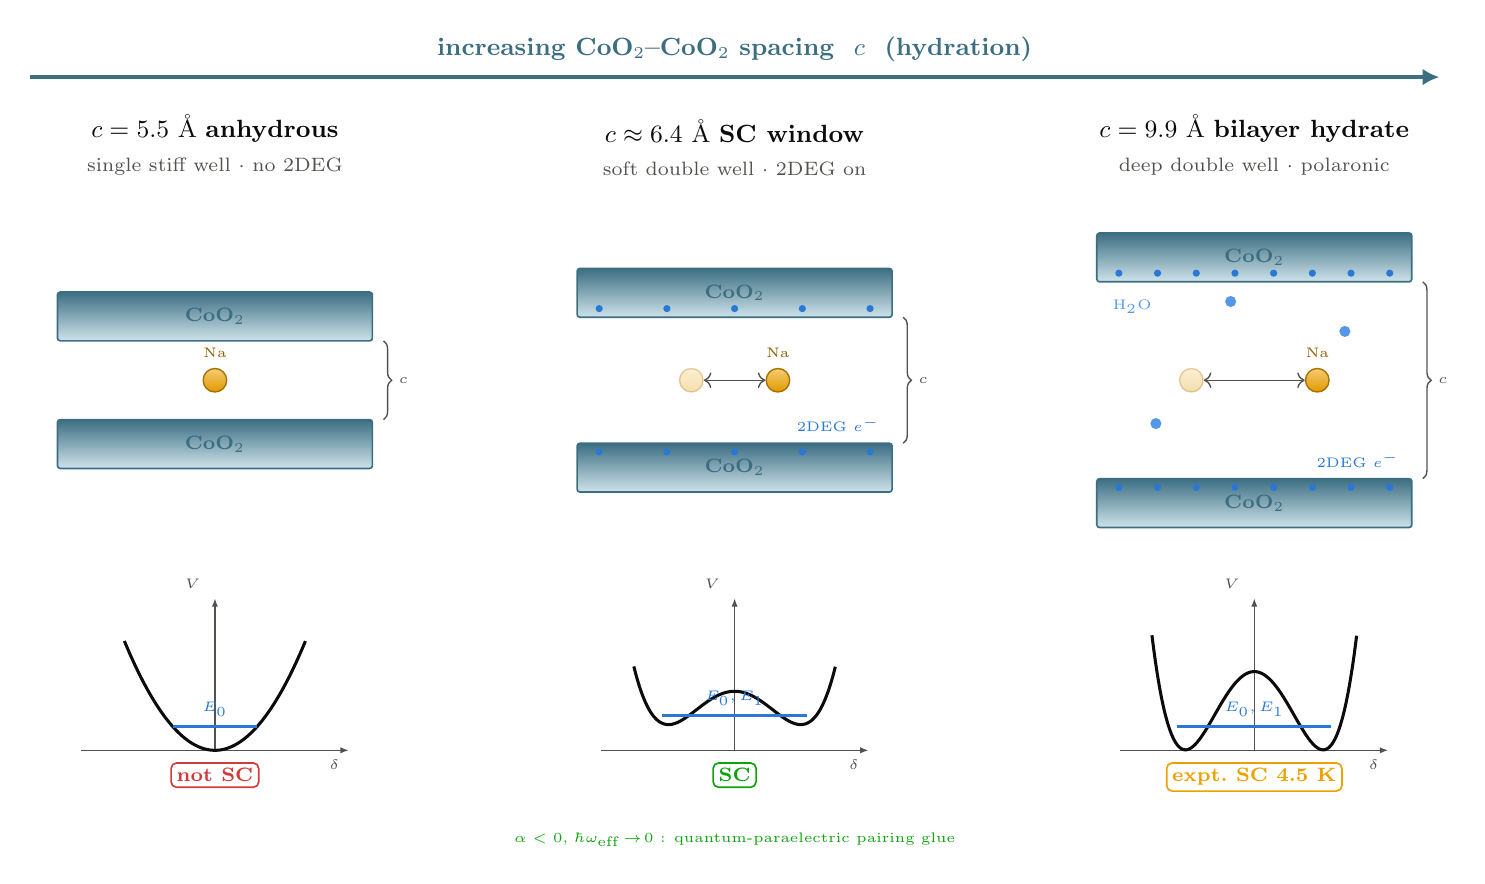
\begin{tikzpicture}[
    font=\sffamily,
    slabstyle/.style={draw=slab,line width=0.6pt,top color=slab,
        bottom color=slablt,rounded corners=1pt},
    naion/.style={circle,draw=na!70!black,line width=0.5pt,
        top color=na!55,bottom color=na!95!black,minimum size=8.5pt,
        inner sep=0pt},
    elec/.style={circle,fill=egas,inner sep=0pt,minimum size=2.6pt},
  ]

  \def\W{2.0}          % half slab width
  \def\hs{0.62}        % slab thickness
  \def\dx{6.6}         % stage pitch

  % ============================================================= STAGES
  % Crystals are centred on the gallery mid-plane (y=0) so all three stay
  % symmetric as the spacing grows -- titles above / wells below never collide.
  % #1 gap  #2 Na-displacement  #3 n_elec(2DEG)  #4 water?  #5 x-origin
  \foreach \g/\disp/\ne/\wat/\ox/\stg in {
      1.00/0/0/0/0/A, 1.60/0.55/5/0/\dx/B, 2.50/0.80/8/1/{2*\dx}/C}{
    \begin{scope}[shift={(\ox,0)}]
      \pgfmathsetmacro\hg{\g/2}            % half-gap; gallery mid at y=0

      % --- CoO2 slabs (bottom below, top above the gallery) ---
      \fill[slabstyle] (-\W,-\hg-\hs) rectangle (\W,-\hg);
      \fill[slabstyle] (-\W,\hg) rectangle (\W,\hg+\hs);
      \node[slab,font=\scriptsize\bfseries] at (0,-\hg-\hs/2) {CoO$_2$};
      \node[slab,font=\scriptsize\bfseries] at (0,\hg+\hs/2) {CoO$_2$};

      % --- 2DEG: electron sheet on the gallery-facing surfaces ---
      \ifnum\ne>0
        \foreach \k in {1,...,\ne}{
          \pgfmathsetmacro\ex{-\W+0.28+ (\k-1)*(2*\W-0.56)/(\ne-1)}
          \node[elec] at (\ex,-\hg-0.11){};
          \node[elec] at (\ex,\hg+0.11){};
        }
        \node[egas,font=\tiny,anchor=east] at (\W-0.04,-\hg+0.24)
          {2DEG $e^-$};
      \fi

      % --- Na ion (+ bistable ghost + arrow for the double well) ---
      \ifdim\disp pt>0pt
        \node[naion,opacity=0.32] at (-\disp,0){};
        \draw[<->,sec,line width=0.5pt] (-\disp+0.16,0) -- (\disp-0.16,0);
      \fi
      \node[naion] (na\stg) at (\disp,0){};
      \node[na!60!black,font=\tiny,anchor=south] at (\disp,0.17){Na};

      % --- water molecules for the bilayer hydrate ---
      \ifnum\wat>0
        \foreach \wx/\wy in {-1.25/-0.55, 1.15/0.62, -0.30/1.00}{
          \node[circle,fill=water,inner sep=0pt,minimum size=4pt]
            at (\wx,\wy){};
          \fill[white] (\wx-0.11,\wy+0.06) circle (0.9pt);
          \fill[white] (\wx+0.11,\wy+0.06) circle (0.9pt);
        }
        \node[water,font=\tiny,anchor=west] at (-\W+0.08,\hg-0.32){H$_2$O};
      \fi

      % --- spacing brace on the right ---
      \draw[decorate,decoration={brace,amplitude=3pt},sec,line width=0.5pt]
        (\W+0.14,\hg) -- (\W+0.14,-\hg)
        node[midway,anchor=west,font=\tiny,sec,xshift=2pt]{$c$};
    \end{scope}
  }

  % ============================================================= WELLS
  % mini potential V(delta) under each stage: single / soft-double / deep-double
  \def\wy{-3.05}       % well-plot baseline (top of frame)
  \def\ww{1.55}        % well half-width
  \def\wh{1.65}        % well height
  \foreach \ox/\type/\lvl in {0/single/1, \dx/soft/2, {2*\dx}/deep/3}{
    \begin{scope}[shift={(\ox,\wy)}]
      % frame axes
      \draw[sec,line width=0.5pt,-{Latex[length=3pt]}]
        (-\ww-0.15,-\wh) -- (\ww+0.15,-\wh);      % delta axis
      \draw[sec,line width=0.5pt,-{Latex[length=3pt]}]
        (0,-\wh) -- (0,0.28);                     % V axis
      \node[sec,font=\tiny,anchor=north east] at (\ww+0.15,-\wh){$\delta$};
      \node[sec,font=\tiny,anchor=south east] at (-0.06,0.28){$V$};

      \ifnum\lvl=1  % ---- stiff single well ----
        \draw[ink,line width=1.1pt,smooth,domain=-1.15:1.15,samples=60]
          plot (\x,{-\wh + 1.05*\x*\x});
        \pgfmathsetmacro\ea{-\wh+0.30}
        \draw[egas,line width=1.0pt] (-0.53,\ea)--(0.53,\ea);
        \node[egas,font=\tiny,anchor=south] at (0,\ea+0.01){$E_0$};
      \fi
      \ifnum\lvl=2  % ---- soft double well ----
        \draw[ink,line width=1.1pt,smooth,domain=-1.28:1.28,samples=80]
          plot (\x,{-\wh + 0.75 + (-1.20*\x*\x + 0.85*\x*\x*\x*\x)});
        \pgfmathsetmacro\eb{-\wh+0.44}
        \draw[egas,line width=1.0pt] (-0.92,\eb)--(0.92,\eb);
        \node[egas,font=\tiny,anchor=south] at (0,\eb+0.01){$E_0,E_1$};
      \fi
      \ifnum\lvl=3  % ---- deep double well ----
        \draw[ink,line width=1.1pt,smooth,domain=-1.30:1.30,samples=90]
          plot (\x,{-\wh + 1.00 + (-2.60*\x*\x + 1.70*\x*\x*\x*\x)});
        \pgfmathsetmacro\ec{-\wh+0.30}
        \draw[egas,line width=1.0pt] (-0.98,\ec)--(0.98,\ec);
        \node[egas,font=\tiny,anchor=south] at (0,\ec+0.01){$E_0,E_1$};
      \fi
    \end{scope}
  }

  % ============================================================= LABELS
  \def\ty{2.9}         % stage-title baseline
  \foreach \ox/\ttl/\sub/\vd/\vc in {
      0/{$c=5.5$ \AA\ \textbf{anhydrous}}/{single stiff well $\cdot$ no 2DEG}/{not SC}/crit,
      \dx/{$c\approx6.4$ \AA\ \textbf{SC window}}/{soft double well $\cdot$ 2DEG on}/{SC}/good,
      {2*\dx}/{$c=9.9$ \AA\ \textbf{bilayer hydrate}}/{deep double well $\cdot$ polaronic}/{expt.\ SC 4.5 K}/amber}{
    \node[ink,font=\small,anchor=south] at (\ox,\ty){\ttl};
    \node[sec,font=\scriptsize,anchor=south] at (\ox,\ty-0.42){\sub};
    \node[\vc,font=\scriptsize\bfseries,anchor=north,
          draw=\vc,rounded corners=2pt,inner sep=2pt,line width=0.6pt]
      at (\ox,\wy-\wh-0.15){\vd};
  }

  % ============================================================= BIG ARROW
  \draw[-{Latex[length=6pt,width=6pt]},slab,line width=1.6pt]
    (-\W-0.35,\ty+0.95) -- ({2*\dx+\W+0.35},\ty+0.95);
  \node[slab,font=\small\bfseries,anchor=south] at (\dx,\ty+1.02)
    {increasing CoO$_2$--CoO$_2$ spacing \ $c$ \ (hydration)};

  % soft-mode / SC-window callout under the middle stage arrow
  \node[good,font=\tiny,anchor=north] at (\dx,\wy-\wh-0.92)
    {$\alpha<0$, $\hbar\omega_{\mathrm{eff}}\!\to\!0$ : quantum-paraelectric pairing glue};

\end{tikzpicture}
\end{document}
